\section{Sequential Task Execution Experiment}
\label{sec:ex}
We conduct a sequential experiment supposing the situations in a household environment.
\figref{demo_all} shows the snapshots of the experiment. Spreading a cloth, wrapping a box with the cloth, carrying the box and a board are executed, activating each local motion with the human aural commands in order.

%% \figref{demo_all_1} shows the first half of the experiment. At \(t=\SI{55}{s}\), the robot stops walking back with feeling the force caused by the cloth, and stretching the cloth by the human and the robot is realized. Then, conducted by the human instructions and the movements, the transportation of flexible objects is executed by the two at \(t=\SI{110}{s}\). From \(t=\SI{115}{s}\), wrapping task of the box is accomplished. Switching the robot motion type from walking mode to manipulating mode by a human voice command and applying the robot motion generation based on the human hand movement, the task is done completely. Ordering the robot to stop moving its arms by voice at \(t=\SI{180}{s}\) and \(t=\SI{230}{s}\), the role is realized to hold the cloth not to be released until the human put tape on it.

%% \begin{figure}[htbp]
%%   \begin{center}
%%     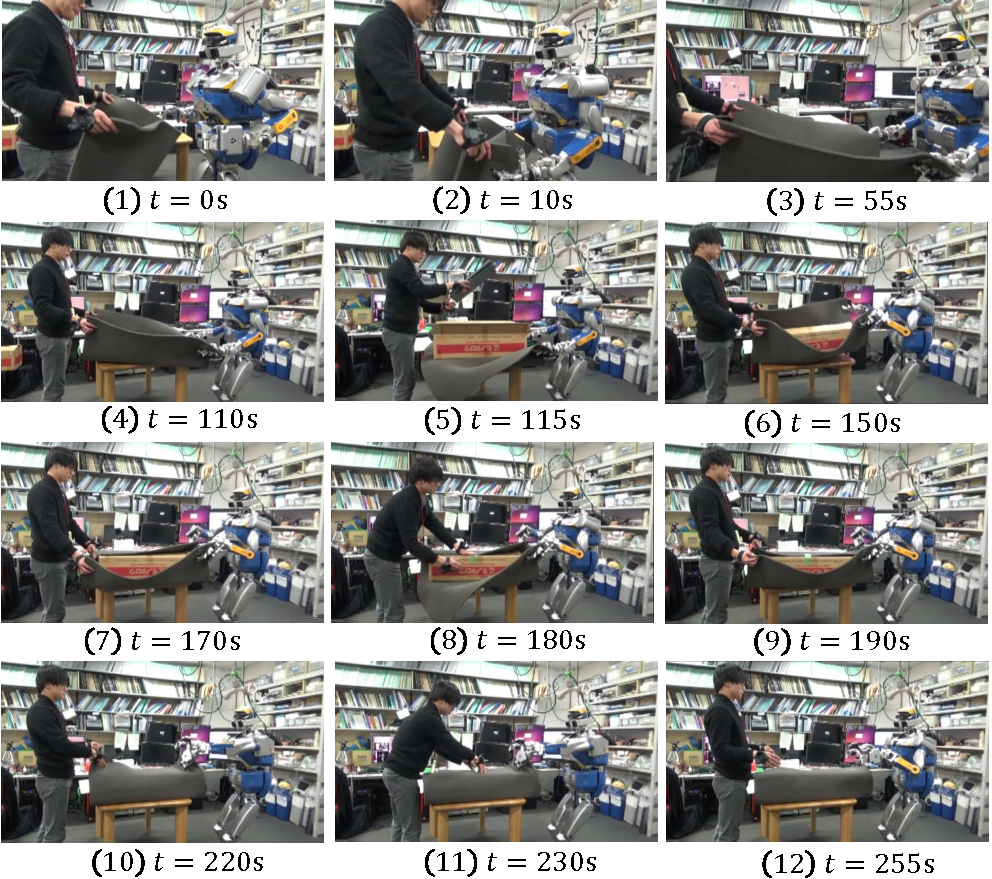
\includegraphics[width=1.00\columnwidth]{figs/demo_all_01}
%%     \caption{The first half of the experiments applying the integrated cooperative system. Stretching the cloth (1)-(3), transporting it (4) and wrapping with it (5)-(12) are executed sequentially. At \(t=\SI{180}{s}\) and \(t=\SI{230}{s}\), the human make the robot stop its motion, and it realizes the role to keep the cloth wrapping the box, not being released.}
%%     \label{figure:demo_all_1}
%%   \end{center}
%% \end{figure}

%% \figref{demo_all_2} shows the latter half of the experiment. It shows that our collaborative carrying methods also works on rigid objects; the box and the board. Applying human velocity and position to generate robot velocity instead of haptic information, sideward transportations that seem to be difficult and aren't executed in the passed works~\cite{aist_cooperative_carrying}\cite{carry_with_vision} are realized.

%% \begin{figure}[htbp]
%%   \begin{center}
%%     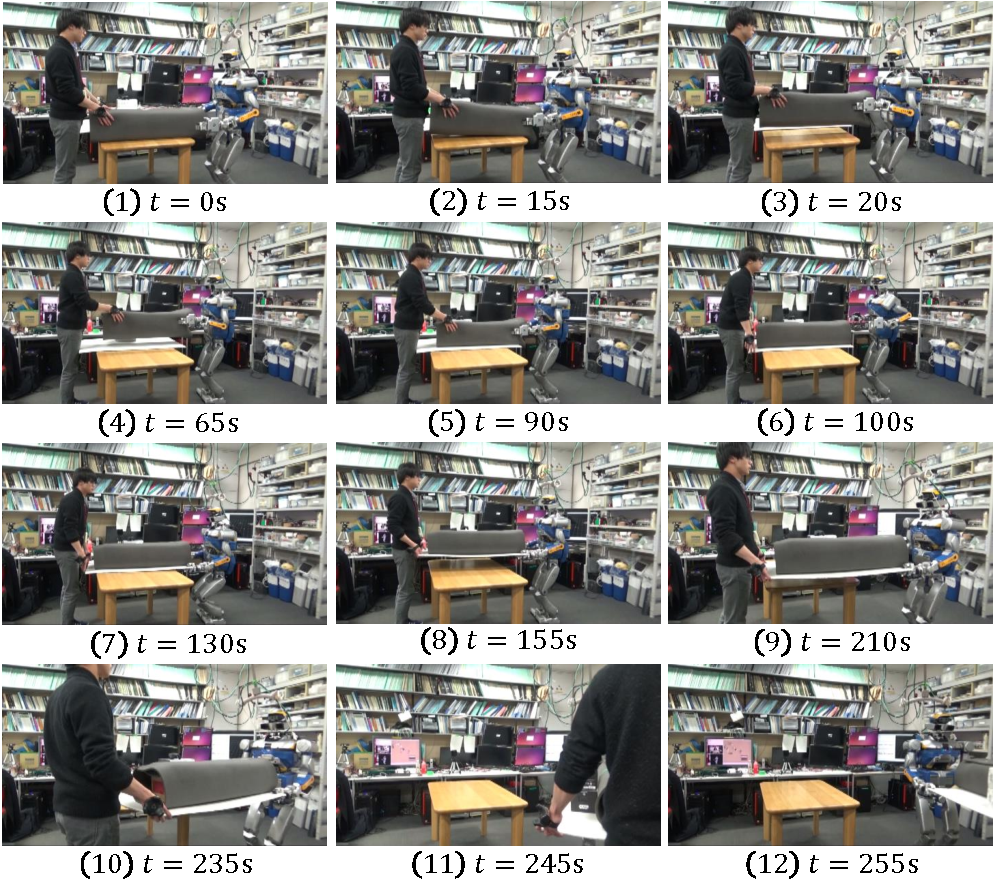
\includegraphics[width=1.00\columnwidth]{figs/demo_all_02}
%%     \caption{The latter half of the experiments applying the integrated cooperative system. Carrying not only flexible objects but also rigid objects is executed through the whole experiment; the box (1)-(5) and the board (6)-(12).}
%%     \label{figure:demo_all_2}
%%   \end{center}
%% \end{figure}

\begin{figure}[htbp]
  \begin{center}
    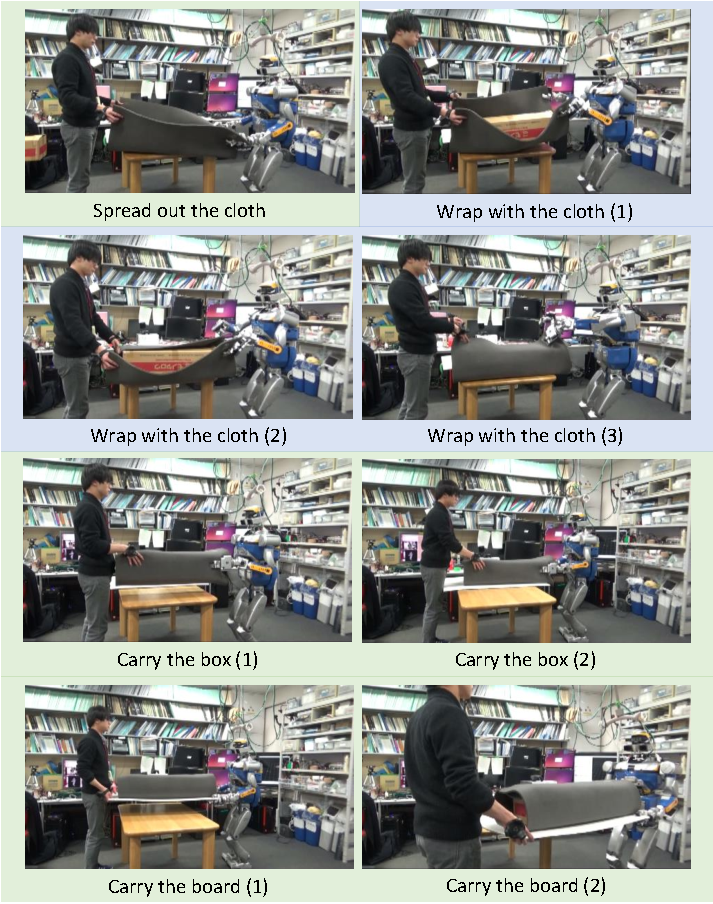
\includegraphics[width=1.00\columnwidth]{figs/demo_all_short}
    \caption{The experiments applying the proposed system. Spreading a cloth, wrapping a box with the cloth, carrying the box and a board are executed. Blue shaded parts and the green shaded parts represent the parts using the local motions described in \subsecref{move_hand} and \subsecref{walk} respectively.}
    \label{figure:demo_all}
  \end{center}
\end{figure}
